\qrchapter{https://forgottenpillar.com/rsc/en-fp-chapter13}{The Sabbath God vs. Sunday God - J. B. Frisbie}


\qrchapter{https://forgottenpillar.com/rsc/es-fp-chapter13}{El Dios del sábado contra el Dios del domingo - J. B. Frisbie}


There are other articles written on the \emcap{personality of God} by our pioneers and it would be too much to include everything here, but we would like to add one more testimony from brother J. B. Frisbie’s article where he compares the Sabbath God with the Sunday God. He compares the truth on the \emcap{personality of God} expressed in the first point of the \emcap{Fundamental Principles} with the Trinity doctrine. Let us take a look at a portion of his article, “\textit{The Seventh Day-Sabbath Not Abolished}” from the Review and Herald, March 7, 1854.


Hay otros artículos escritos sobre la \emcap{personalidad de Dios} por nuestros pioneros y sería demasiado incluir todo aquí, pero nos gustaría añadir un testimonio más del artículo del hermano J. B. Frisbie donde compara al Dios del sábado con el Dios del domingo. Él compara la verdad sobre la \emcap{personalidad de Dios} expresada en el primer punto de los \emcap{Principios Fundamentales} con la doctrina trinitaria. Veamos una porción de su artículo, “\textit{The Seventh Day-Sabbath Not Abolished}” (El séptimo día-sábado no está abolido) de la Review and Herald, 7 de marzo de 1854.


\begin{figure}[hp]
    \centering
    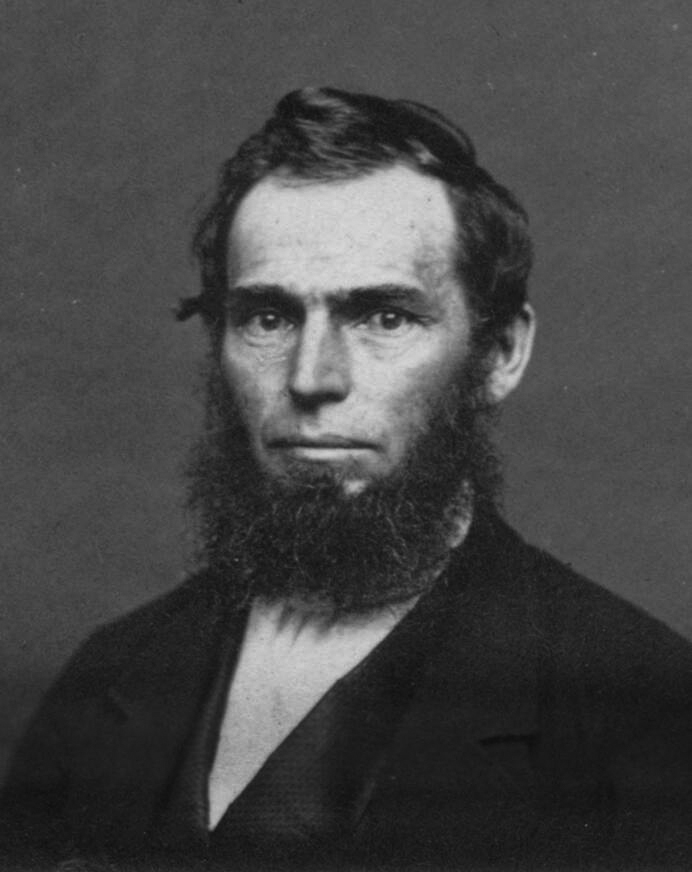
\includegraphics[width=1\linewidth]{images/j-b-frisbie.jpg}
    \caption*{John Byington Frisbie (1816-1882)}
    \label{fig:j-b-frisbie}
\end{figure}


\begin{figure}[hp]
    \centering
    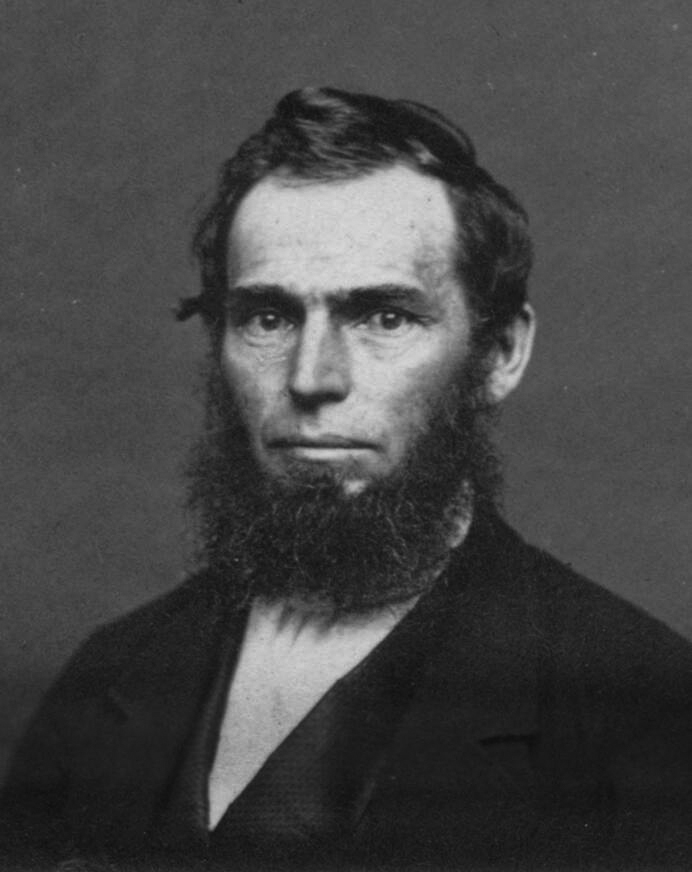
\includegraphics[width=1\linewidth]{images/j-b-frisbie.jpg}
    \caption*{John Byington Frisbie (1816-1882)}
    \label{fig:j-b-frisbie}
\end{figure}


\section*{The Sabbath God}


\section*{El Dios del Sábado}


\others{After we know and remember God, by keeping his holy Sabbath, \textbf{then the Bible will teach of his personality and dwelling place}. \textbf{Man is in the image and likeness of God}. Genesis 1:26. ‘And God said, Let us (speaking to his son) make man in our image, after our likeness’. Chap 2:7. ‘And the Lord God formed man of the dust of the ground, and breathed into his nostrils the breath of life: and man became a living soul’. Genesis 9:6; 1 Corinthians 11:7; James 3:9. \textbf{That which was made in \underline{the image and likeness of God} was made of the dust of the ground called man}.}


\others{Después de que conozcamos y recordemos a Dios, guardando su santo sábado, \textbf{entonces la Biblia nos enseñará sobre su personalidad y morada}. \textbf{El hombre es a imagen y semejanza de Dios}. Génesis 1:26. ‘Y dijo Dios: Hagamos (hablando con su hijo) al hombre a nuestra imagen, conforme a nuestra semejanza’. Capítulo 2:7. ‘Y Jehová Dios formó al hombre del polvo de la tierra, y sopló en su nariz aliento de vida; y fue el hombre un ser viviente’. Génesis 9:6; 1 Corintios 11:7; Santiago 3:9. \textbf{Lo que fue hecho a \underline{la imagen y semejanza de Dios} fue hecho del polvo de la tierra llamado hombre}.}


\othersnogap{This is known to be the true sense from other testimonies that may be given from the Bible. \textbf{Jesus was in the form of a man and the express image of his Father’s person}.}


\othersnogap{Se sabe que este es el verdadero sentido por otros testimonios que se pueden dar de la Biblia. \textbf{Jesús tenía forma de hombre y era la imagen expresa de la persona de su Padre}.}


\othersnogap{Philippians 2:6-8. \textbf{Christ Jesus}: ‘Who, being in \textbf{the form of God}, thought it not robbery to be \textbf{equal with God}. But made himself of no reputation, and took upon him \textbf{the form of a servant}, and was \textbf{made in the likeness of men’}. 2 Corinthians 4:4. \textbf{‘And being formed in fashion as a man’}, etc. Colossians 1:15. ‘\textbf{Who is the image of the invisible God}’.}


\othersnogap{Filipenses 2:6-8. \textbf{Cristo Jesús}: ‘El cual, siendo en \textbf{forma de Dios}, no estimó el ser \textbf{igual a Dios} como cosa a que aferrarse. Sino que se despojó a sí mismo, tomando \textbf{forma de siervo}, y \textbf{hecho semejante a los hombres}’. 2 Corintios 4:4. \textbf{‘Y siendo formado en forma de hombre’}, etc. Colosenses 1:15. ‘\textbf{Él es la imagen del Dios invisible}’.}


\othersnogap{Hebrews 1:3. \textbf{The Son; ‘Who being the brightness of his glory, and the express image of his person’}. In this sense could Jesus say to Philip in truth, ‘He that hath seen me hath seen the Father.’ John 14:9. Some seem to suppose it argues \textbf{against the personality of God, \underline{because he is a Spirit, and say that he is without body, or parts}}. John 4:24. ‘\textbf{God is a Spirit}’. Hebrews 1:7. ‘\textbf{Who maketh his angels spirits}’. \textbf{Who would pretend to say that angels have no bodies or parts because they are spirits}. \textbf{\underline{None the less is God a spiritual being having body and parts as we may learn by his having a dwelling place and because he has and may be seen}}. Exodus 33:23. ‘And I will take away mine hand, and thou shalt\textbf{ see my back parts}, but my \textbf{face shall not be seen}’. Matthew 5:8. ‘Blessed are the pure in heart, for \textbf{they shall see God}’. Hebrews 12:14. ‘Follow peace with all men, and holiness, without which \textbf{no man shall see the Lord}’. Matthew 18:10. ‘That in heaven their angels do \textbf{always behold the face of my Father which is in heaven}’. Matthew 6:9. ‘After this manner therefore pray ye, \textbf{Our Father which art in heaven}’, etc. John 6:38. ‘For I \textbf{came down from heaven} not to do mine own will, but the will of him that sent me’. Chap 16:28. ‘\textbf{I came forth from the Father, and am come into the world}: again I \textbf{leave the world, and go to the Father}’.}


\othersnogap{Hebreos 1:3. \textbf{El Hijo; ‘El cual, siendo el resplandor de su gloria, y la imagen misma de su sustancia’}. En este sentido pudo decir Jesús a Felipe en verdad: ‘El que me ha visto a mí, ha visto al Padre’. Juan 14:9. Algunos parecen suponer que esto argumenta \textbf{en contra de la personalidad de Dios, \underline{porque es un Espíritu, y dicen que no tiene cuerpo ni partes}}. Juan 4:24. ‘\textbf{Dios es un Espíritu}’. Hebreos 1:7. ‘\textbf{Que hace a sus ángeles espíritus}’. \textbf{¿Quién pretendería decir que los ángeles no tienen cuerpo o partes porque son espíritus?} \textbf{\underline{No obstante, Dios es un ser espiritual que tiene cuerpo y partes, como podemos aprender por el hecho de que tiene una morada y porque tiene y puede ser visto}}. Éxodo 33:23. ‘Y quitaré mi mano, y \textbf{verás mis espaldas}, pero mi \textbf{rostro no se verá}’. Mateo 5:8. ‘Bienaventurados los de limpio corazón, porque \textbf{ellos verán a Dios}’. Hebreos 12:14. ‘Seguid la paz con todos, y la santidad, sin la cual \textbf{nadie verá al Señor}’. Mateo 18:10. ‘Que en los cielos sus ángeles \textbf{ven siempre el rostro de mi Padre que está en los cielos}’. Mateo 6:9. ‘Vosotros, pues, oraréis así: \textbf{Padre nuestro que estás en los cielos}’, etc. Juan 6:38. ‘Porque he \textbf{descendido del cielo}, no para hacer mi voluntad, sino la voluntad del que me envió’. Capítulo 16:28. ‘\textbf{Salí del Padre, y he venido al mundo}; otra vez \textbf{dejo el mundo, y voy al Padre}’.}


\othersnogap{\textbf{Does not God say he fills immensity of space? \underline{We answer, No}}. Psalm 139:7, 8. ‘Whither shall I go \textbf{from thy Spirit}? or whither shall I flee \textbf{from thy presence}? If I ascend up into heaven, thou art there’, etc. \textbf{\underline{God by his Spirit may fill heaven and earth}}, etc. \textbf{Some confound God with his Spirit, which makes confusion}. Psalm 11:4. ‘\textbf{The Lord is in his holy temple, the Lord’s throne is in heaven}: his eyes behold’, etc. Habakkuk 2:20; Psalm 102:19. ‘For he hath looked \textbf{down from the height of his Sanctuary}; \textbf{\underline{from heaven} did the Lord behold the earth’}. 1 Peter 3:12. ‘For the eyes of the Lord are over the righteous, and his ears are open unto their prayers’, etc. Psalm 80:1. ‘Give ear, O Shepherd of Israel, thou that leadest Joseph like a flock; thou \textbf{that dwellest between the cherubims}, shine forth’. Psalm 99:1; Isaiah 37:16.}


\othersnogap{\textbf{¿No dice Dios que llena la inmensidad del espacio? \underline{Respondemos que no}}. Salmo 139:7, 8. ‘¿Adónde me iré \textbf{de tu Espíritu}? ¿O adónde huiré \textbf{de tu presencia}? Si subo a los cielos, allí estás tú’, etc. \textbf{\underline{Dios por su Espíritu puede llenar el cielo y la tierra}}, etc. \textbf{Algunos confunden a Dios con su Espíritu, lo que crea confusión}. Salmo 11:4. ‘\textbf{Jehová está en su santo templo; Jehová tiene en el cielo su trono}; sus ojos ven’, etc. Habacuc 2:20; Salmo 102:19. ‘Porque miró \textbf{desde lo alto de su santuario}; \textbf{\underline{desde los cielos} miró Jehová a la tierra}’. 1 Pedro 3:12. ‘Porque los ojos del Señor están sobre los justos, y sus oídos atentos a sus oraciones’, etc. Salmo 80:1. ‘Oh Pastor de Israel, escucha, tú que pastoreas como a ovejas a José; \textbf{tú que estás entre querubines}, resplandece’. Salmo 99:1; Isaías 37:16.}


\othersnogap{John 14:2. ‘In my Father’s house are many mansions. I go to prepare a place for you’. Revelation 21:2-5; Hebrews 11:6. ‘For he that cometh to God must believe that he is’, etc. \textbf{This testimony we deem highly important at this time, to know that there is a God. We have no doubt that if our eyes could be opened in vision, or see as angels see, we should see God in heaven sitting on his throne, and is present to all that exists, however distant from him in his creation}.}[\href{https://documents.adventistarchives.org/Periodicals/RH/RH18540307-V05-07.pdf}{Adventist Review and Sabbath Herald, March 7, 1854}, J. B. Frisbie, “The Seventh-Day Sabbath Not Abolished”, p. 50]


\othersnogap{Juan 14:2. ‘En la casa de mi Padre muchas moradas hay. Voy, pues, a preparar lugar para vosotros’. Apocalipsis 21:2-5; Hebreos 11:6. ‘Porque es necesario que el que se acerca a Dios crea que le hay’, etc. \textbf{Este testimonio lo consideramos muy importante en este momento, para saber que hay un Dios. No dudamos de que si nuestros ojos pudieran abrirse en visión, o ver como ven los ángeles, veríamos a Dios en el cielo sentado en su trono, y está presente a todo lo que existe, por muy distante que esté de él en su creación}.}[\href{https://documents.adventistarchives.org/Periodicals/RH/RH18540307-V05-07.pdf}{Adventist Review and Sabbath Herald, March 7, 1854}, J. B. Frisbie, “The Seventh-Day Sabbath Not Abolished”, p. 50]


Here we see the same argument and reasoning, that God is a personal spiritual Being. This God is the Sabbath God. Brother Frisbie compares this God with the Sunday God, who is a trinitarian God.


Aquí vemos el mismo argumento y razonamiento, que Dios es un Ser espiritual personal. Este Dios es el Dios del sábado. El hermano Frisbie compara a este Dios con el Dios dominical, que es un Dios trinitario.


\section*{The Sunday God}


\section*{El Dios dominical}


\others{We will make a few extracts, that the reader may \textbf{see the broad contrast between \underline{the God of the Bible} brought to light through Sabbath-keeping, and the god in the dark through Sunday-keeping}. Catholic Catechism Abridged by the Rt. Rev. John Dubois, Bishop of New York. Page 5. ‘\textbf{Ques. Where is God? Ans. God is everywhere}. Q. Does God see and know all things? A. Yes, he does know and see all things. \textbf{Q. Has God any body? A. \underline{No; God has no body, he is a pure Spirit}}. \textbf{Q. Are there more Gods than one? A. No; there is but one God. Q. Are there more persons than one in God? A. \underline{Yes; in God there are three persons}. Q. Which are they? A. God the Father, God the Son and God the Holy Ghost. Q. Are there not three Gods? A. No; the Father, the Son and the Holy Ghost, are all but one and the same God}’.}


\others{Haremos unos pocos extractos, para que el lector pueda \textbf{ver el amplio contraste entre \underline{el Dios de la Biblia} sacado a la luz a través de la observancia del sábado, y el dios en la oscuridad a través de la observancia del domingo}. Catecismo Católico, abreviado por el Reverendo John Dubois, Obispo de Nueva York. Página 5. ‘\textbf{Pregunta. ¿Dónde está Dios? Respuesta. Dios está en todas partes}. P. ¿Ve y conoce Dios todas las cosas? R. Sí, conoce y ve todas las cosas. \textbf{P. ¿Tiene Dios algún cuerpo? R. \underline{No; Dios no tiene cuerpo, es un Espíritu puro}}. \textbf{P. ¿Hay más dioses que uno? R. No, sólo hay un Dios. P. ¿Hay más personas que una en Dios? R. \underline{Sí; en Dios hay tres personas}. P. ¿Cuáles son? R. Dios Padre, Dios Hijo y Dios Espíritu Santo. P. ¿No hay tres Dioses? R. No; el Padre, el Hijo y el Espíritu Santo no son más que un mismo Dios}’.}


\othersnogap{The first article of the Methodist Religion, p. 8. \textbf{‘There is but one living and true God}, everlasting, \textbf{without body or parts}, of infinite power, wisdom and goodness: the maker and preserver of all things, visible and invisible. \textbf{And in unity of this God-head, there are three persons of one substance, power and eternity; the Father, the Son, and the Holy Ghost}.’}


\othersnogap{El primer artículo de la Religión Metodista, p. 8. \textbf{‘No hay más que un solo Dios vivo y verdadero}, eterno, \textbf{sin cuerpo ni partes}, de infinito poder, sabiduría y bondad: el hacedor y preservador de todas las cosas, visibles e invisibles. \textbf{Y en la unidad de este Dios-cabeza, hay tres personas de una sola sustancia, poder y eternidad: el Padre, el Hijo y el Espíritu Santo}’.}


\othersnogap{In this article like the Catholic doctrine, \textbf{we are taught that there are three persons of one substance,} power and eternity making\textbf{ in all one living and true God}, everlasting \textbf{without body or parts}. But in all this we are not told \textbf{what became of the body of Jesus who had a body when he ascended, who went to God who ‘is everywhere’ or nowhere}. Doxology.}


\othersnogap{En este artículo, al igual que la doctrina católica, \textbf{se nos enseña que hay tres personas de una sola sustancia,} poder y eternidad que hacen\textbf{ en todo un solo Dios vivo y verdadero}, eterno \textbf{sin cuerpo ni partes}. Pero en todo esto no se nos dice \textbf{qué fue del cuerpo de Jesús que tenía cuerpo cuando ascendió, que fue a Dios que ‘está en todas partes’ o en ninguna}. Doxología.}


\othersnogap{‘\textbf{To God the Father, God the Son,}} \\
\others{\textbf{God the Spirit, three in one.}’} \\
\others{Again} \\
\others{‘Warms in the sun, refreshes in the breeze,} \\
\others{Glows in the stars, and blossoms in the trees.} \\
\others{\textbf{Lives through all life, extends through all extent},} \\
\others{Spreads undivided and operates unspent.’ - Pope.}


\othersnogap{‘\textbf{A Dios Padre, Dios Hijo,}} \\
\others{\textbf{Dios Espíritu, tres en uno}’} \\
\others{Otra vez} \\
\others{‘Calienta en el sol, refresca en la brisa,} \\
\others{Brilla en las estrellas, y florece en los árboles.} \\
\others{\textbf{Vive a través de toda la vida, se extiende a través de toda la extensión},} \\
\others{Se extiende sin división y opera sin gasto’. - Papa.}


\othersnogap{These ideas well accord with those heathen philosophers. One says, ‘That water was the principle of all things, and that God is that intelligence, by whom all things are formed out of water.’ Another, ‘That air is God, that it is produced, that it is immense and infinite,’ etc. A third, ‘That God is a soul diffused throughout all beings of nature,’ etc. \textbf{Some, who had the idea of \underline{a pure Spirit}}. Last of all, ‘That God is an eternal substance.’}


\othersnogap{Estas ideas concuerdan bien con aquellos filósofos paganos. Uno dice: ‘Que el agua era el principio de todas las cosas, y que Dios es esa inteligencia, por la que todas las cosas son formadas a partir del agua’. Otro, ‘Que el aire es Dios, que es producido, que es inmenso e infinito’, etc. Un tercero, ‘Que Dios es un alma difundida en todos los seres de la naturaleza’, etc. \textbf{Algunos, que tenían la idea de \underline{un Espíritu puro}}. Por último, ‘Que Dios es una sustancia eterna’.}


\othersnogap{These extracts are taken from Rollin’s History, Vol. II, pp. 597-8, published by Harpers. \textbf{We should rather mistrust that the Sunday god came from the same source that Sunday-keeping did}. ‘Sunday was a name given by the heathens to the first day of the week, because it was the day on which they worshiped the sun.’ - Union Bible Dictionary. \textbf{Afterward modified by the Roman Catholic Church, in the form we now find it taught through the land}.}


\othersnogap{Estos extractos están tomados de la Historia de Rollin, vol. II, pp. 597-8, publicada por Harpers. \textbf{Deberíamos desconfiar más bien de que el dios del domingo provenga de la misma fuente que la observancia del domingo}. ‘El domingo era un nombre dado por los paganos al primer día de la semana, porque era el día en que adoraban al sol’. - Diccionario bíblico de la unión. \textbf{Posteriormente fue modificado por la Iglesia Católica Romana, en la forma que ahora encontramos que se enseña en toda la tierra}.}


\othersnogap{It is very natural to suppose when \textbf{the Pope set himself up to be God in the temple of God}, [2 Thessalonians 2:4] that he should have a day sanctified to his worship. This he has done. - Douay Catechism, p. 59. ‘Q. What is the best means to sanctify Sunday? A. By hearing mass, etc. This saying mass is for the priest to gabble over Latin, drink some wine, and give the people a wafer to eat.’}”“\others{But God sanctified his day because he had rested on it. Another day for a very different purpose. Genesis 2:3.}


\othersnogap{Es muy natural suponer que cuando \textbf{el Papa se erigió en Dios en el templo de Dios}, [2 Tesalonicenses 2:4] debía tener un día santificado para su culto. Esto es lo que ha hecho. - Catecismo de Douay, p. 59. ‘P. ¿Cuál es el mejor medio para santificar el domingo? R. Oyendo misa, etc. Este decir misa es para que el sacerdote parlotee sobre el latín, beba un poco de vino y dé al pueblo una hostia para comer’.}”“\others{Pero Dios santificó su día porque había descansado en él. Otro día para un propósito muy diferente. Génesis 2:3.}


\othersnogap{In days before the moral fall of Babylon God directed the minds of his honest children right in their prayers, whatever they might think at other times, but now since the apostasy the mind reaches to no god but to the people only, there are many prayers to men we know by their effect and eloquence. \textbf{We are truly thankful to our heavenly Father that \underline{he has led our minds from such folly}, to know, and remember \underline{his holy name} by keeping his holy day that we might love, serve and worthily \underline{glorify him through our great High Priest in the heavenly Sanctuary in this day of atonement}}.}[Ibid.][https://documents.adventistarchives.org/Periodicals/RH/RH18540307-V05-07.pdf]


\othersnogap{En los días anteriores a la caída moral de Babilonia, Dios dirigía las mentes de sus honrados hijos correctamente en sus oraciones, independientemente de lo que pensaran en otros momentos, pero ahora, desde la apostasía, la mente no alcanza a ningún dios, sino sólo al pueblo, hay muchas oraciones a los hombres que conocemos por su efecto y elocuencia. \textbf{Estamos verdaderamente agradecidos a nuestro Padre celestial porque \underline{ha guiado nuestras mentes de tal locura}, para conocer y recordar \underline{su santo nombre} guardando su día santo para que podamos amarlo, servirlo y \underline{glorificarlo dignamente por medio de nuestro gran Sumo Sacerdote en el Santuario celestial en este día de expiación}}.}[Ibid.][https://documents.adventistarchives.org/Periodicals/RH/RH18540307-V05-07.pdf]


Before becoming a Seventh-day Adventist, Frisbie was a Methodist preacher and a bitter opponent of Adventist beliefs. In 1853, after a debate on the Sabbath with Joseph Bates, he reversed his position and began to keep the Sabbath and preach the Seventh-day Adventist doctrine. He renounced Sunday, the Trinity, and accepted the Seventh-day Sabbath and the truth about God, that the Seventh-day Adventist’s taught in the first point of the \emcap{Fundamental Principles}.


Antes de convertirse en adventista del séptimo día, Frisbie era un predicador metodista y un amargo oponente de las creencias adventistas. En 1853, tras un debate sobre el sábado con Joseph Bates, cambió su posición y comenzó a guardar el sábado y a predicar la doctrina adventista del séptimo día. Renunció al domingo, a la trinidad, y aceptó el sábado del séptimo día y la verdad sobre Dios, que los adventistas del séptimo día enseñaban en el primer punto de los \emcap{Principios Fundamentales}.


Do other Adventist pioneers see discordance between the Trinity doctrine and the \emcap{personality of God} expressed in the first point of the \emcap{Fundamental Principles}?


¿Otros pioneros adventistas ven discordancia entre la doctrina trinitaria y la \emcap{personalidad de Dios} expresada en el primer punto de los \emcap{Principios Fundamentales}?


% The Sabbath God vs. Sunday God - J. B. Frisbie

\begin{titledpoem}
    \stanza{
        On seventh day or first we kneel, \\
        But deeper truths these days reveal. \\
        Not just when we choose to pray, \\
        But which God we serve each day.
    }

    \stanza{
        The Sabbath God, a Being clear, \\
        With form and place, both far and near. \\
        In His image we were made, \\
        His Son the perfect likeness displayed. \\
    }

    \stanza{
        The Son, the Father's image bright, \\
        Shows us the path to truth and light. \\
        "Who's seen me has seen the Father too," \\
        Christ's words both powerful and true.
    }

    \stanza{
        The Sunday God, a trinity, \\
        Three persons in strange unity. \\
        Without body, without part, \\
        A concept born from human art.
    }

    \stanza{
        One God with face and hands and form, \\
        Who rested when creation's storm \\
        Had ceased its work on seventh day, \\
        This God commands we rest and pray.
    }

    \stanza{
        Not some essence spreading wide, \\
        Formless spirit with no side. \\
        But a Person on a throne, \\
        With His Son, yet not alone.
    }

    \stanza{
        So choose not merely when to kneel, \\
        But which God your heart finds real. \\
        The day we keep reveals our view \\
        Of which God we believe is true.
    }
\end{titledpoem}


% \qrchapter{https://forgottenpillar.com/rsc/pl-fp-chapter13}{Bóg szabatu a Bóg niedzieli — J. B. Frisbie}

Istnieją inne artykuły na temat \emcap{osobowości Boga} napisane przez naszych pionierów i trudno byłoby zawrzeć tu wszystkie, ale chcielibyśmy dodać jeszcze jedno świadectwo z artykułu brata J. B. Frisbie’go, w którym porównuje on Boga szabatu z Bogiem niedzieli. Porównuje on prawdę o \emcap{osobowości Boga} wyrażoną w pierwszym punkcie \emcap{Fundamentalnych Zasad} z doktryną o Trójcy. Przyjrzyjmy się fragmentowi jego artykułu „\textit{Szabat dnia siódmego nie zniesiony}” z \textit{Review and Herald} z 7 marca 1854 roku.

\begin{figure}[hp]
    \centering
    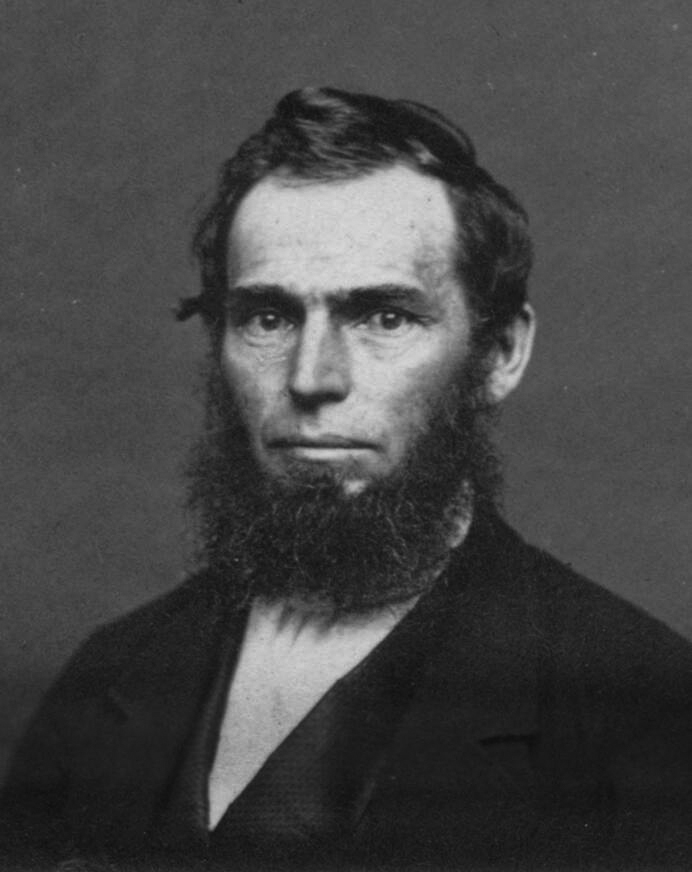
\includegraphics[width=1\linewidth]{images/j-b-frisbie.jpg}
    \caption*{John Byington Frisbie (1816-1882)}
    \label{fig:j-b-frisbie}
\end{figure}


\section*{Bóg szabatu}

\others{Gdy poznamy Boga i będziemy o Nim pamiętać, przestrzegając Jego świętego szabatu, \textbf{wtedy Biblia nauczy nas o Jego osobowości i miejscu zamieszkania}. \textbf{Człowiek jest na obraz i podobieństwo Boga}. Rdz 1:26. «I rzekł Bóg: Uczyńmy (mówiąc do swojego syna) człowieka na nasz obraz, według naszego podobieństwa». Rozdz. 2:7. «I ukształtował Pan Bóg człowieka z prochu ziemi, i tchnął w jego nozdrza tchnienie życia. I stał się człowiek duszą żyjącą». Rdz 9:6; 1Kor 11:7; Jk 3:9. \textbf{To, co zostało stworzone na \underline{obraz i podobieństwo Boga}, zostało uczynione z prochu ziemi i nazwane człowiekiem}.}

\othersnogap{To jest uznawane za prawdziwe znaczenie na podstawie innych świadectw, które można znaleźć w Biblii. \textbf{Jezus był w postaci człowieka i dokładnym obrazem osoby swojego Ojca}.}

\othersnogap{Flp 2:6--8. \textbf{Chrystus Jezus}: «Który, będąc w \textbf{postaci Boga}, nie uważał za grabież być \textbf{równym Bogu}. Lecz ogołocił samego siebie i przyjął \textbf{postać sługi}, i \textbf{został uczyniony na podobieństwo ludzi}». 2Kor 4:4. \textbf{«A będąc ukształtowany na wzór człowieka»}... Kol 1:15. «\textbf{Który jest obrazem niewidzialnego Boga}».}

\othersnogap{Hbr 1:3. \textbf{Syn; «Który, będąc jasnością jego chwały i dokładnym obrazem jego osoby»}. W tym sensie Jezus mógł zgodnie z prawdą powiedzieć do Filipa: «Kto mnie widział, widział i Ojca». J 14:9. Niektórzy wydają się sądzić, że \textbf{przeczy to osobowości Boga, \underline{ponieważ jest On Duchem, i mówią, że nie ma On ciała ani części ciała}}. J 4:24. «\textbf{Bóg jest duchem}». Hbr 1:7. «\textbf{Który czyni swoich aniołów duchami}». \textbf{Kto ośmieliłby się twierdzić, że aniołowie nie mają ciał ani części ciała, ponieważ są duchami}? \textbf{\underline{Niemniej jednak Bóg jest istotą duchową posiadającą ciało i części ciała, o czym dowiadujemy się przez to, że ma miejsce zamieszkania, i ponieważ można go zobaczyć}}. Wj 33:23. «I odejmę moją rękę, i \textbf{ujrzysz moje plecy}, ale \textbf{moje oblicze nie będzie widziane}». Mt 5:8. «Błogosławieni czystego serca, albowiem \textbf{oni zobaczą Boga}». Hbr 12:14. «Dążcie do pokoju ze wszystkimi i do świętości, bez której \textbf{nikt nie ujrzy Pana}». Mt 18:10. «Że w niebie ich aniołowie \textbf{zawsze patrzą na oblicze mojego Ojca, który jest w niebie}». Mt 6:9. «Wy więc tak się módlcie: \textbf{Ojcze nasz, który jesteś w niebie}»... J 6:38. «Bo \textbf{zstąpiłem z nieba} nie po to, żeby czynić swoją wolę, lecz wolę tego, który mnie posłał». Rozdz. 16:28. «\textbf{Wyszedłem od Ojca i przyszedłem na świat}; znowu \textbf{opuszczam świat i idę do Ojca}».}

\othersnogap{\textbf{Czy Bóg nie mówi, że wypełnia nieskończoność przestrzeni? \underline{Odpowiadamy: Nie}}. Ps 139:7, 8. «Dokąd ujdę przed \textbf{twoim duchem}? I dokąd ucieknę przed \textbf{twoją obecnością}? Jeśli wstąpię do nieba, ty tam jesteś»... \textbf{\underline{Bóg przez swojego Ducha może wypełniać niebo i ziemię}}. \textbf{Niektórzy mylą Boga z Jego Duchem, co prowadzi do zamieszania}. Ps 11:4. «\textbf{Pan jest w swoim świętym przybytku, tron Pana jest w niebie}: jego oczy patrzą...». Ha 2:20; Ps 102:19. «Bo spojrzał \textbf{w dół z wysokości swojej świątyni}; \textbf{\underline{z nieba} Pan popatrzył na ziemię»}. 1P 3:12. «Oczy Pana są nad sprawiedliwymi, a jego uszy otwarte są na ich modlitwy...». Ps 80:1. ‘Słuchaj, Pasterzu Izraela, ty, który prowadzisz Józefa jak stado; ty, \textbf{który mieszkasz między cherubinami}, zajaśniej». Ps 99:1; Iz 37:16.}

\othersnogap{J 14:2. «W domu mego Ojca jest wiele posiadłości. Idę przygotować miejsce dla was». Obj 21:2--5; Hbr 11:6. «Bo kto przychodzi do Boga, musi wierzyć, że on jest...». \textbf{To świadectwo uważamy za niezwykle ważne w tym czasie, ażeby wiedzieć, iż jest Bóg. Nie mamy wątpliwości, że gdyby nasze oczy mogły zostać otwarte w wizji lub widzieć tak, jak widzą aniołowie, zobaczylibyśmy Boga w niebie siedzącego na swoim tronie, i jest On obecny we wszystkim, co istnieje, bez względu na to, jak daleko od Niego w Jego stworzeniu}.}[\href{https://documents.adventistarchives.org/Periodicals/RH/RH18540307-V05-07.pdf}{Adventist Review and Sabbath Herald, 7 marca 1854}, J. B. Frisbie, “The Seventh-Day Sabbath Not Abolished”, str. 50]

Tutaj widzimy ten sam argument i rozumowanie, że Bóg jest osobową istotą duchową. Ten Bóg jest Bogiem szabatu. Brat Frisbie porównuje tego Boga z Bogiem niedzieli, który jest Bogiem trynitarnym.

\section*{Bóg niedzieli}

\others{Przedstawimy kilka fragmentów, aby czytelnik mógł \textbf{zobaczyć wyraźny kontrast między \underline{Bogiem Biblii} ujawnionym na światło przez zachowywanie szabatu, a bogiem w ciemności przez zachowywanie niedzieli}. Skrócona wersja katechizmu Kościoła katolickiego autorstwa Wielebnego Johna Dubois, Biskupa Nowego Jorku. Strona 5. «\textbf{Pyt. Gdzie jest Bóg? Odp. Bóg jest wszędzie}. P. Czy Bóg widzi i wie wszystko? O. Tak, On wie i widzi wszystko. \textbf{P. Czy Bóg ma ciało? O. \underline{Nie; Bóg nie ma ciała, jest jedynie Duchem}}. \textbf{P. Czy jest więcej Bogów niż jeden? O. Nie; jest tylko jeden Bóg. P. Czy jest więcej osób niż jedna w Bogu? O. \underline{Tak; w Bogu są trzy osoby}. P. Które to są? O. Bóg Ojciec, Bóg Syn i Bóg Duch Święty. P. Czy nie ma trzech Bogów? O. Nie; Ojciec, Syn i Duch Święty to wszystko jeden i ten sam Bóg}».}

\othersnogap{Pierwszy artykuł Religii Metodystycznej, str. 8. \textbf{«Jest tylko jeden żywy i prawdziwy Bóg}, wieczny, \textbf{bez ciała i części ciała}, o nieskończonej mocy, mądrości i dobroci: stwórca i zachowawca wszystkich rzeczy, widzialnych i niewidzialnych. \textbf{A w jedności tego Bóstwa są trzy osoby jednej substancji, mocy i wieczności; Ojciec, Syn i Duch Święty}.’}

\othersnogap{W tym artykule, podobnie jak w doktrynie katolickiej, \textbf{uczy się nas, że są trzy osoby jednej substancji}, mocy i wieczności tworzące \textbf{w sumie jednego żywego i prawdziwego Boga}, wiecznego \textbf{bez ciała i części ciała}. Ale w tym wszystkim nie powiedziano nam, \textbf{co stało się z ciałem Jezusa, który miał ciało, gdy wstąpił do nieba, który poszedł do Boga, który ‘jest wszędzie» albo nigdzie}. Doksologia.}

\othersnogap{«\textbf{Bogu Ojcu, Bogu Synowi,}} \\
\others{\textbf{Trzem w jednym i Bogu Duchowi}».} \\
\others{Znowu} \\
\others{«Grzeje w słońcu, orzeźwia w powiewie,} \\
\others{Świeci w gwiazdach i kwitnie na drzewie.} \\
\others{\textbf{Wypełnia wszelkie życie, bezkres obejmuje},} \\
\others{Niesie się niepodzielnie i się nie wyczerpuje». — Papież.}

\othersnogap{Te idee dobrze współgrają z poglądami filozofów pogańskich. Jeden mówi, «że woda była podstawą wszystkich rzeczy, a Bóg jest tą duchową istotą, przez którą wszystkie rzeczy są kształtowane z wody». Inny, «że powietrze jest Bogiem, że jest wytwarzane, że jest niezmierzone i nieskończone...». Trzeci, «że Bóg jest duszą przenikającą wszystkie byty natury...». \textbf{Niektórzy wyznają ideę \underline{wyłącznie Ducha}}. I wreszcie, «że Bóg jest wieczną substancją».}

\othersnogap{Te fragmenty są wzięte z \textit{The Ancient History} autorstwa Rollina, tom II, str. 597--598, wydanej przez Harpers. \textbf{Nie powinniśmy raczej wierzyć, że bóg niedzieli pochodzi z tego samego źródła co zachowywanie niedzieli}. «Niedziela (Sunday) była nazwą nadaną przez pogan pierwszemu dniowi tygodnia, ponieważ był to dzień, w którym czcili słońce (the sun)». — The Union Bible Dictionary. \textbf{Później została zmodyfikowana przez Kościół rzymskokatolicki do postaci, w jakiej obecnie jest nauczana w całym kraju}.}

\othersnogap{Bardzo naturalne jest przypuszczenie, że gdy \textbf{Papież ustanowił się Bogiem w świątyni Bożej} [2Tes 2:4], musiał mieć dzień poświęcony dla swojej czci. To właśnie uczynił. — Douay, Katechizm, str. 59. «P. Jaki jest najlepszy sposób na uświęcenie niedzieli? O. Między innymi przez słuchanie mszy. To odprawianie mszy polega na tym, że ksiądz mamrocze po łacinie, pije wino i daje ludziom opłatek do zjedzenia».} \others{Ale Bóg uświęcił swój dzień, ponieważ w nim odpoczął. Inny dzień do zupełnie innego celu. Rdz 2:3.}

\othersnogap{W dniach przed moralnym upadkiem Babilonu Bóg zwracał umysły swoich szczerych dzieci we właściwym kierunku w ich modlitwach, bez względu na to, co mogłyby myśleć w innych chwilach, ale teraz od czasu odstępstwa umysł nie dociera do żadnego boga, tylko do ludzi, jest wiele modlitw do ludzi, które rozpoznajemy po ich wpływie i elokwencji. \textbf{Jesteśmy prawdziwie wdzięczni naszemu niebiańskiemu Ojcu, że \underline{wyprowadził nasze umysły z takiego szaleństwa}, abyśmy poznali i pamiętali \underline{Jego święte imię} przez zachowywanie Jego świętego dnia, abyśmy mogli Go kochać, służyć Mu i godnie \underline{Go chwalić przez naszego wielkiego Arcykapłana w niebiańskiej Świątyni w tym dniu pojednania}}.}[Tamże.][https://documents.adventistarchives.org/Periodicals/RH/RH18540307-V05-07.pdf]

Zanim został adwentystą dnia siódmego, Frisbie był kaznodzieją metodystycznym i zagorzałym przeciwnikiem wierzeń adwentystycznych. W 1853 roku, po debacie na temat szabatu z Josephem Batesem, zmienił swoje stanowisko i zaczął zachowywać szabat oraz głosić doktrynę Adwentystów Dnia Siódmego. Wyrzekł się niedzieli, Trójcy i przyjął prawdę o szabacie dnia siódmego oraz prawdę o Bogu, której Adwentyści Dnia Siódmego nauczali w pierwszym punkcie \emcap{Fundamentalnych Zasad}.

Czy inni pionierzy adwentyzmu dostrzegają niezgodność między doktryną o Trójcy a \emcap{osobowością Boga} wyrażoną w pierwszym punkcie \emcap{Fundamentalnych Zasad}?

% Bóg szabatu a Bóg niedzieli - J. B. Frisbie

\begin{titledpoem}

    \stanza{
        Dwa obrazy Boga, dwie różne natury, \\
        Jeden prawdą jaśnieje, drugi w cieniu bury. \\
        Bóg szabatu osobą z ciałem i częściami, \\
        Bóg niedzieli bezkształtny, rozlany nad światami.
    }

    \stanza{
        Na obraz Stwórcy człowiek uformowany, \\
        Z prochu ziemi przez Boga mądrze ukształtowany. \\
        Syn jest obrazem Ojca, doskonałym odbiciem, \\
        Kto widział Syna, Ojca ujrzał z zachwytem.
    }

    \stanza{
        Bóg ma tron w niebie, miejsce przebywania, \\
        Przez Ducha swego wszędzie jest od zarania. \\
        Nie jest On wszędzie obecny w swej istocie, \\
        Lecz przez Ducha działa w każdej życia dobrocie.
    }

\end{titledpoem}

\begin{titledpoem}

    \stanza{
        Szabat czy niedziela – więcej niż dzień tygodnia, \\
        To wyznanie wiary, co duszę rozpogadnia. \\
        Szabat wskazuje na Boga osobowego, \\
        Niedziela na bóstwo z pogaństwa wyjętego.
    }

    \stanza{
        Bóg szabatu ma ciało, ma oblicze swoje, \\
        Syn Jego jest obrazem, nie jakąś częścią troje. \\
        Bóg niedzieli to "trzech w jednym" bez ciała, \\
        Doktryna, którą filozofia pogańska znała.
    }

    \stanza{
        Jeden Bóg prawdziwy na tronie zasiada, \\
        Drugi wszędzie i nigdzie, jak mgła się rozkłada. \\
        Wybór dnia świętego to wybór Boga twego, \\
        Kogo czcisz naprawdę? Osobę czy coś mglistego?
    }

\end{titledpoem}

\begin{titledpoem}

    \stanza{
        Frisbie odkrył prawdę, gdy szabat przyjmował, \\
        Od metodystów odszedł, Trójcę odrzutował. \\
        Poznał Boga Biblii, nie boga tradycji, \\
        Znalazł prawdę czystą, bez ludzkiej kompozycji.
    }

    \stanza{
        Bóg ma ciało duchowe, ma swoje mieszkanie, \\
        Przez Syna objawia swoje panowanie. \\
        Nie jest On substancją bez formy i kształtu, \\
        Lecz Osobą, co godna czci i zachwytu.
    }

    \stanza{
        Dzień siódmy czy pierwszy – to nie tylko data, \\
        To wyznanie, kogo dusza twa uważa za Brata. \\
        Boga, który stworzył i odpoczął potem, \\
        Czy bóstwo wymyślone ludzkim umysłem i słowem.
    }
    
\end{titledpoem}

